\chapter{Locomotion Controller Transfer from Virtual To Real World}
\section{Motivation}
Robotics and character animation share a common goal, to design locomotion controllers, the algorithmic ``brain'' that allow animated characters and robots to move naturally, robustly and efficiently in a complex dynamic environment. Despite this commonality, there is a gap between the state-of-the-art of these two fields. While in character animation, we have demonstrated that it is possible to control a full humanoid character to perform challenging locomotion tasks in a physically simulated environment, we have not yet seen any robots that have comparable capabilities. For example, controlling human walking is considered as a solved problem in character animation, but it is still an open research in robotics. In addition, we have demonstrated in the previous Chapters that with the powerful computational tools, controller can be optimized autonomously in a virtual environment. However, in robotics, designing controllers is still a challenging, trial-and-error process that is limited only to highly-specialized engineers. Can we extend the computational tools developed for character animations to robotics to close the gap between these two fields?

One major challenge to directly applying the methods we have developed to control robots is the Reality Gap: Controllers that work effectively for a virtual character in the simulation may perform poorly on a robot in the real environment. The most important factors that lead to the Reality Gap include hardware limitation, unmodelled dynamics, inaccurate physical properties, noise and latency. For example, the torque limits of the servos on the robot are seldom considered in animation applications. We also do not model the dynamics of the servos. Even though we often can acquire the physical properties, such as mass, center of mass and inertia, of a robot from its CAD files, they are usually inaccurate given the manufacturing error, assembly error and the cables that are not considered in CAD files. Furthermore, the noise in the environment and the latency in hardware communication also contribute to the Reality Gap.

To cross the Reality Gap and to design robotic controllers autonomously, we develop a system with three components, physical simulation, controller optimization and simulation calibration. We first build a physical simulation of articulated rigid bodies to model the dynamics of the robot and its environment. Different from the simulators used in animation, we incorporate the torque limits, servo dynamics, noise and latency measured from the robot experiments into our simulator. We then optimize a controller for a specific locomotion task in the physical simulation. However, if we apply this optimal controller directly to the robot, it will fail the task in the real world due to the Reality Gap. To solve this problem, we collect the real performance data, and use it to calibrate our physical simulator. We optimize a set of simulation parameters, including the mass, inertia, center of mass and actuator gains of the robot, to minimize the discrepancy between the simulation results and the collected real data. Through calibration, the simulator can capture the real world dynamics more faithfully. This calibrated simulator is used again in controller optimization to improve the quality of the controller. Depending on the task, it could take several iterations of simulation calibration and controller optimization to transfer the controller to the real robot. 

We evaluate our system in three locomotion tasks, rising from a leaning, sitting, or kneeling position to an erect stance. These motions are widely used in our daily life. Although most of us can perform them with ease, it is a big challenge for some elderly persons and patients with hamspring injuries. We choose to study these motions and synthesize them on robots due to these important health-care applications. One simple solution to achieve these tasks is to use static balance. The robot increases the area of the contact polygon by establishing more contact points, and then rises its body slowly while maintaining the COM within the contact polygon. We choose not to use this strategy because in real life, we human can perform these motions in a more agile fashion, and we hope that our controller can enable robots to demonstrate comparable agility. For this reason, our controllers will utilize impulsive actions and take advantage of the dynamic motion to rise. In addition, since one main contribution of our method is simulation calibration, to best test its effectiveness, we only use feedforward controllers in our evaluations. In contrast, if feedback controllers are used, the stability region of the task would be drastically increased, which makes the simulation accuracy less critical. Our results show that simulation calibration is effective. In most cases, only one iteration of calibration is needed to transfer the controller successfully to the real robot. Our system is able to design locomotion controllers autonomously, which work successfully both in the simulation and in the real world. 

\section{Overview}

\begin{figure}[!t]
  \centering
  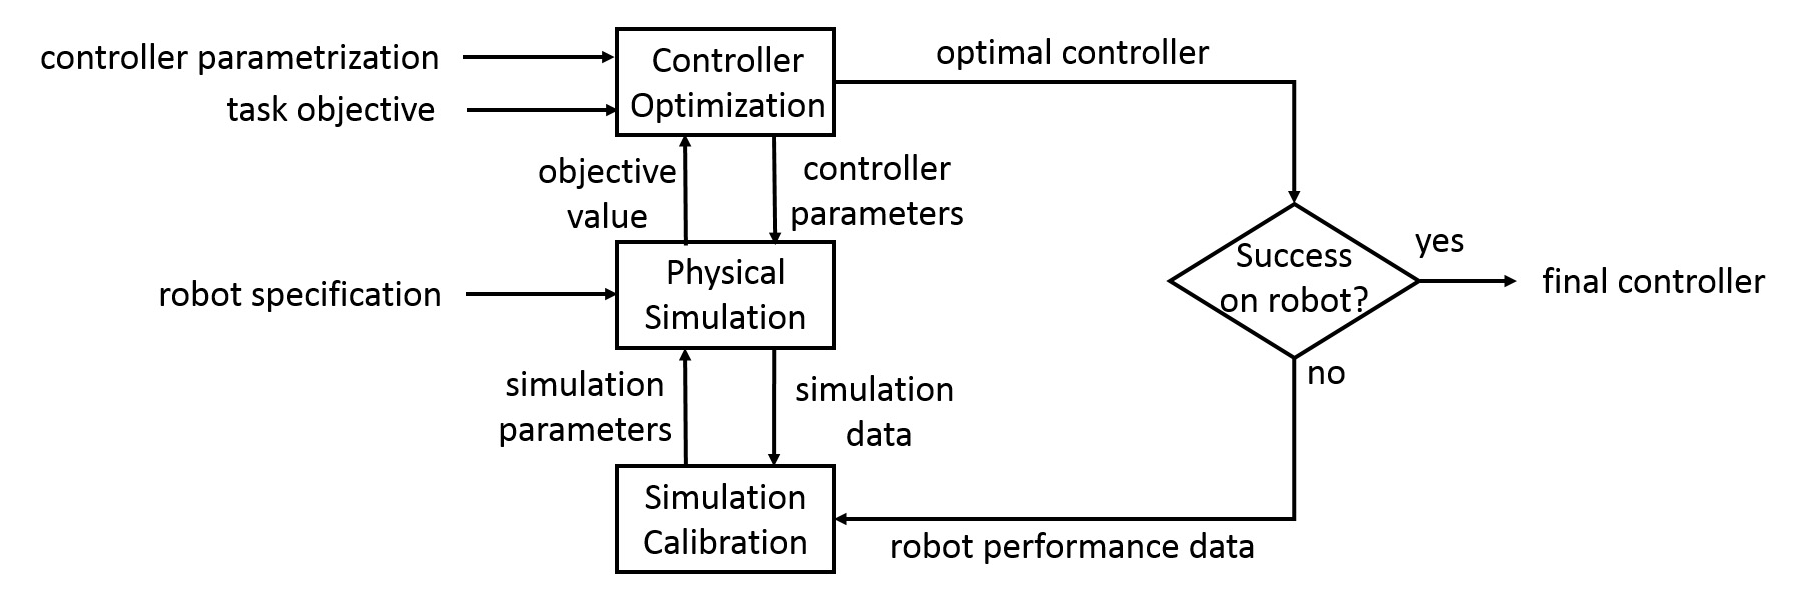
\includegraphics[width=6in]{figures/controllerTransfer}
  \caption{Overview of our algorithm.}
  \label{fig:controllerTransferOverview}
\end{figure}

We have designed a system that can automatically design locomotion controllers for robots (Figure~\ref{fig:controllerTransferOverview}). Given the specification of the robot, including its body shape, the physical properties of each body, and the types of joints, we build a physical simulation using Dynamic Animation and Robotics Toolkit (DART) \cite{dart:2012}, an open source articulated rigid body simulator. In addition, we also take into consideration the torque limits, servo gains, noise and latency, which are not modeled in DART. The controller optimization subsystem runs thousands of simulations to search for the optimal controller to minimize the task-related objective function. We then test this optimal controller on the robot. If the robot successfully completes the task, a working robotic controller is found and our algorithm terminates. Otherwise, we record the robot performance data and feed it into the simulation calibration subsystem. Simulation calibration runs another optimization, which searches for the optimal simulation parameters to minimize the discrepancy between the performance data from the simulation and that from the robot experiments. The loop of controller optimization and simulation calibration is performed iteratively until the controller works successfully on the real robot. In the next three sections, we will delve into the details of these main components of our system, physical simulation, controller optimization and system calibration.

\section{Physical Simulation}

\subsection{Dynamics Equations}

We model the robot as an articulated rigid body system in our simulator. We represent the states of the system $(\mathbf{x}, \dot{\mathbf{x}})$ in the generalized coordinate, where $\mathbf{x}$ include the global position $\mathbf{p}$, orientation $\mathbf{r}$ of the root link, and the joint angles $\mathbf{q}$. We solve the governing equations of motion eq.(\ref{eq:robotdynamics}) in the generalized coordinates.

\begin{equation}
\label{eq:robotdynamics}
\mathbf{M}(\mathbf{x})\mathbf{\ddot{x}}+\mathbf{C}(\mathbf{x},\mathbf{\dot{x}})=\mathbf{\tau}+\mathbf{Jf}
\end{equation}
where $\mathbf{M}(\mathbf{x})$ is the mass matrix and $\mathbf{C}(\mathbf{x},\mathbf{\dot{x}})$ is the Coriolis and Centrifugal force. $\mathbf{\tau}$ are joint torques exerted by the actuators. $\mathbf{J}$ is the Jacobian matrix and $\mathbf{f}$ is the external contact force, which is computed based on linear complementarity conditions. In our implementation, we use DART to solve eq.(\ref{eq:robotdynamics}) along with the contact forces.

\subsection{Actuator Model}

In character animations, joint torques $\tau$ are often chosen as the control signal since they can be directly integrated in eq.(\ref{eq:robotdynamics}). However, the control signal for the robot that we use in the experiments, ROBOTIS BIOLOID GP, is the desired angle $\bar{q}$ for each joint. Given difference between desired and current joint configuration ${q-\bar{q}}$, the actual servo first maps it to a corresponding power level $U$ and eventually outputs joint torque according to the internal actuator dynamics.

\begin{figure}[t]
\centering
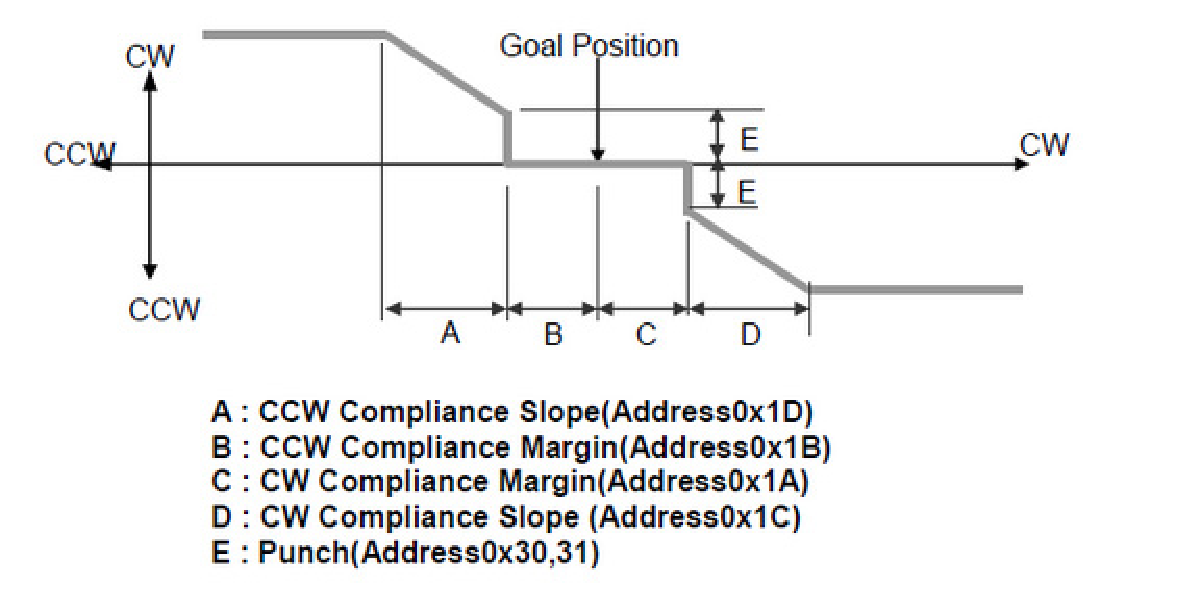
\includegraphics[width=5in]{figures/ax18gain.eps}
\caption{The mapping between $q-\bar{q}$ and $U$ for a AX-18 motor \cite{AX18:2015}. The x-axis is $q-\bar{q}$ while the y-axis is $U$.}
\label{fig:actuatorMap}
\end{figure}

Most of the actuators on our robot are AX-18, which use the following mapping (Figure \ref{fig:actuatorMap}) between the joint angle difference $q-\bar{q}$ and the power level $U$. The inteval A and C determine the slope of the actuator response for clock-wise and counter-clock-wise motions respectively. Smaller values mean steeper response slopes, in which case the actuator follows the desired angle more closely. However, too small values can lead to overshooting problems. B and D are compliance margin. If the servo angle has only a small difference to the desired angle, specified by B and D, the servo shuts down and outputs zero torque. E, the punch, is the minimum power level before the servo shuts down. In practice, we set A and C to be the same so that the servo will behave the same no matter it rotates clock-wise or counter-clock-wise. In addition, since B, D and E are very small compared to A and C, we ignore their effects and approximate the mapping as a linear relation with slope $k_e$:
\begin{equation}
  U=k_e(q-\bar{q})
  \label{eqn:voltageErrorRelation}
\end{equation}

We adopt a model for the ideal DC motor \cite{SchwarzB:2013} to derive the relation between power level $U$ and output torque $\tau$. The assumption of using an ideal model is good since an AX-18 servo contain a high-quality DC motor. The derivation follows by considering the power balance present in the motor at a constant voltage U:
\begin{equation}
  P_{electric} = P_{mechanic} + P_{heat}
  \label{eqn:powerBalance}
\end{equation}
where $P_{electric}$ is the electrical power, $P_{mechanic}$ is the output mechanical power and $P_{heat}$ is the power dissipated as heat. From eq.(\ref{eqn:powerBalance}), we can get the following relation:
\begin{equation}
UI=\dot{q}\tau_{motor} + RI^2
\end{equation}
where $I$ is the current and $R$ is the motor winding resistance. Rearrange the above equation and plugging into the relation between $\tau$ and $I$, $\tau_{motor}=k_{\tau}I$, we arrive at the relation between $U$ and the torque generated by the motor:
\begin{equation}
  U=k_{\tau}\dot{q}+\frac{R}{k_{\tau}}\tau_{motor}
  \label{eqn:votageTorqueRelation}
\end{equation}
where $k_{\tau}$ is the torque constant, which is determined by the hardware design of the motor. The torque generated by the DC motor usually does not equal the output torque that drives the motor shaft due to the friction inside the motor. The total torque is converted into the output torque $\tau$ and the friction torque $\tau_f$.
\begin{equation}
  \tau_{motor}=\tau+\tau_f
  \label{eqn:torqueBalance}
\end{equation}
The friction torque can be further divided into viscous friction and Coulomb friction \cite{SchwarzB:2013}:
\begin{equation}
  \tau_f = -k_v\dot{q}-k_c\sgn(\dot{q})
  \label{eqn:frictionComponents}
\end{equation}
where $k_v$ and $k_c$ are friction coefficients for the viscous and Coulomb friction respectively. $\sgn(x)$ is the sign function that equals 1 if x is positive, -1 if x is negative and 0 otherwise.

Combining eq.(\ref{eqn:votageTorqueRelation}), (\ref{eqn:torqueBalance}) and (\ref{eqn:frictionComponents}), we arrive at the relation between the joint angle error $q-\bar{q}$ and the output torque $\tau$.
\begin{align}
\nonumber  \tau & = \frac{k_{\tau}k_e}{R}(q-\bar{q})+(k_v-\frac{k_{\tau}^2}{R})\dot{q}+k_c\sgn(\dot{q})\\
\nonumber & = k_p(q-\bar{q}) + k_d\dot{q} + k_c\sgn(\dot{q})\\
  \label{eqn:torqueErrorRelationSimple}
\end{align}
where $k_p=\frac{k_{\tau}k_e}{R}$ and $k_d=k_v-\frac{k_{\tau}^2}{R}$. We call these values $k_p$, $k_d$ and $k_c$ \emph{actuator gains}. Note that it is possible to compute actuator gains if the related parameters are given in the specification sheet of the motor. However, this information is not available for the motors that we use. In Chapter 6.6, we will show how to design experiments to measure these parameters. Plugging eq.(\ref{eqn:torqueErrorRelationSimple}) into (\ref{eq:robotdynamics}), and taking torque limits $[\tau_{min}, \tau_{max}]$ into consideration, we get the dynamics equation that use the reference joint motion as the control signal.
\begin{displaymath}
 \mathbf{M}(\mathbf{x})\mathbf{\ddot{x}}+\mathbf{C}(\mathbf{x},\mathbf{\dot{x}}) = \tau+\mathbf{Jf} \\
  \end{displaymath}
where 
\begin{displaymath}\tau =
  \left\{
    \begin{array}{ll}
      \tau_{min} & \text{if }\tau < \tau_{min},\\
      \tau_{max} & \text{if }\tau > \tau_{max},\\
      k_p(\mathbf{q}-\bar{\mathbf{q}}) + k_d\dot{\mathbf{q}} + k_c\sgn(\dot{\mathbf{q}}) & \text{otherwise.}\\
    \end{array}
  \right.
  \label{eqn:robotDynamicsControl}
\end{displaymath}

To guarantee the stability of the simulation, we use 1ms as the simulation time step. Many animation system use the same simulation and control frequency, which means that a control signal $\bar{\mathbf{q}}$ is updated every simulation time step. However, we find that the average latency of the whole control loop on our robot is 16ms, including the time to send actuator commands and to read sensor measurements through the serial port. To better match our simulation with the real robot situation, we choose to only update the control signal every 16 time steps.

\section{Controller Optimization}

Given the physical simulation, we can design controllers to enable the robot achieve various locomotion tasks in the simulated environment. The three tasks are rising from leaning, sitting and kneeling position to an erect stance (Figure \ref{fig:task}). For each task, the joint configuration of the initial pose and the final pose are provided by the user. The goal of the controller is to execute a sequence of control signals so that the robot can move from the initial to the final pose without losing balance. We purposefully choose to use only feedforward controllers in this work. Without feedback control, the controller transfer will not succeed even if the simulation and the real-world environment differ greatly. This can put the simulation calibration subsystem into a more thorough test. For this reason, the control signal $\bar{\mathbf{q}}(t)$ is a only function of time $t$ and does not depend on the states of the robot $\mathbf{x}$ and $\dot{\mathbf{x}}$.

\begin{figure}[!t]
  \centering
  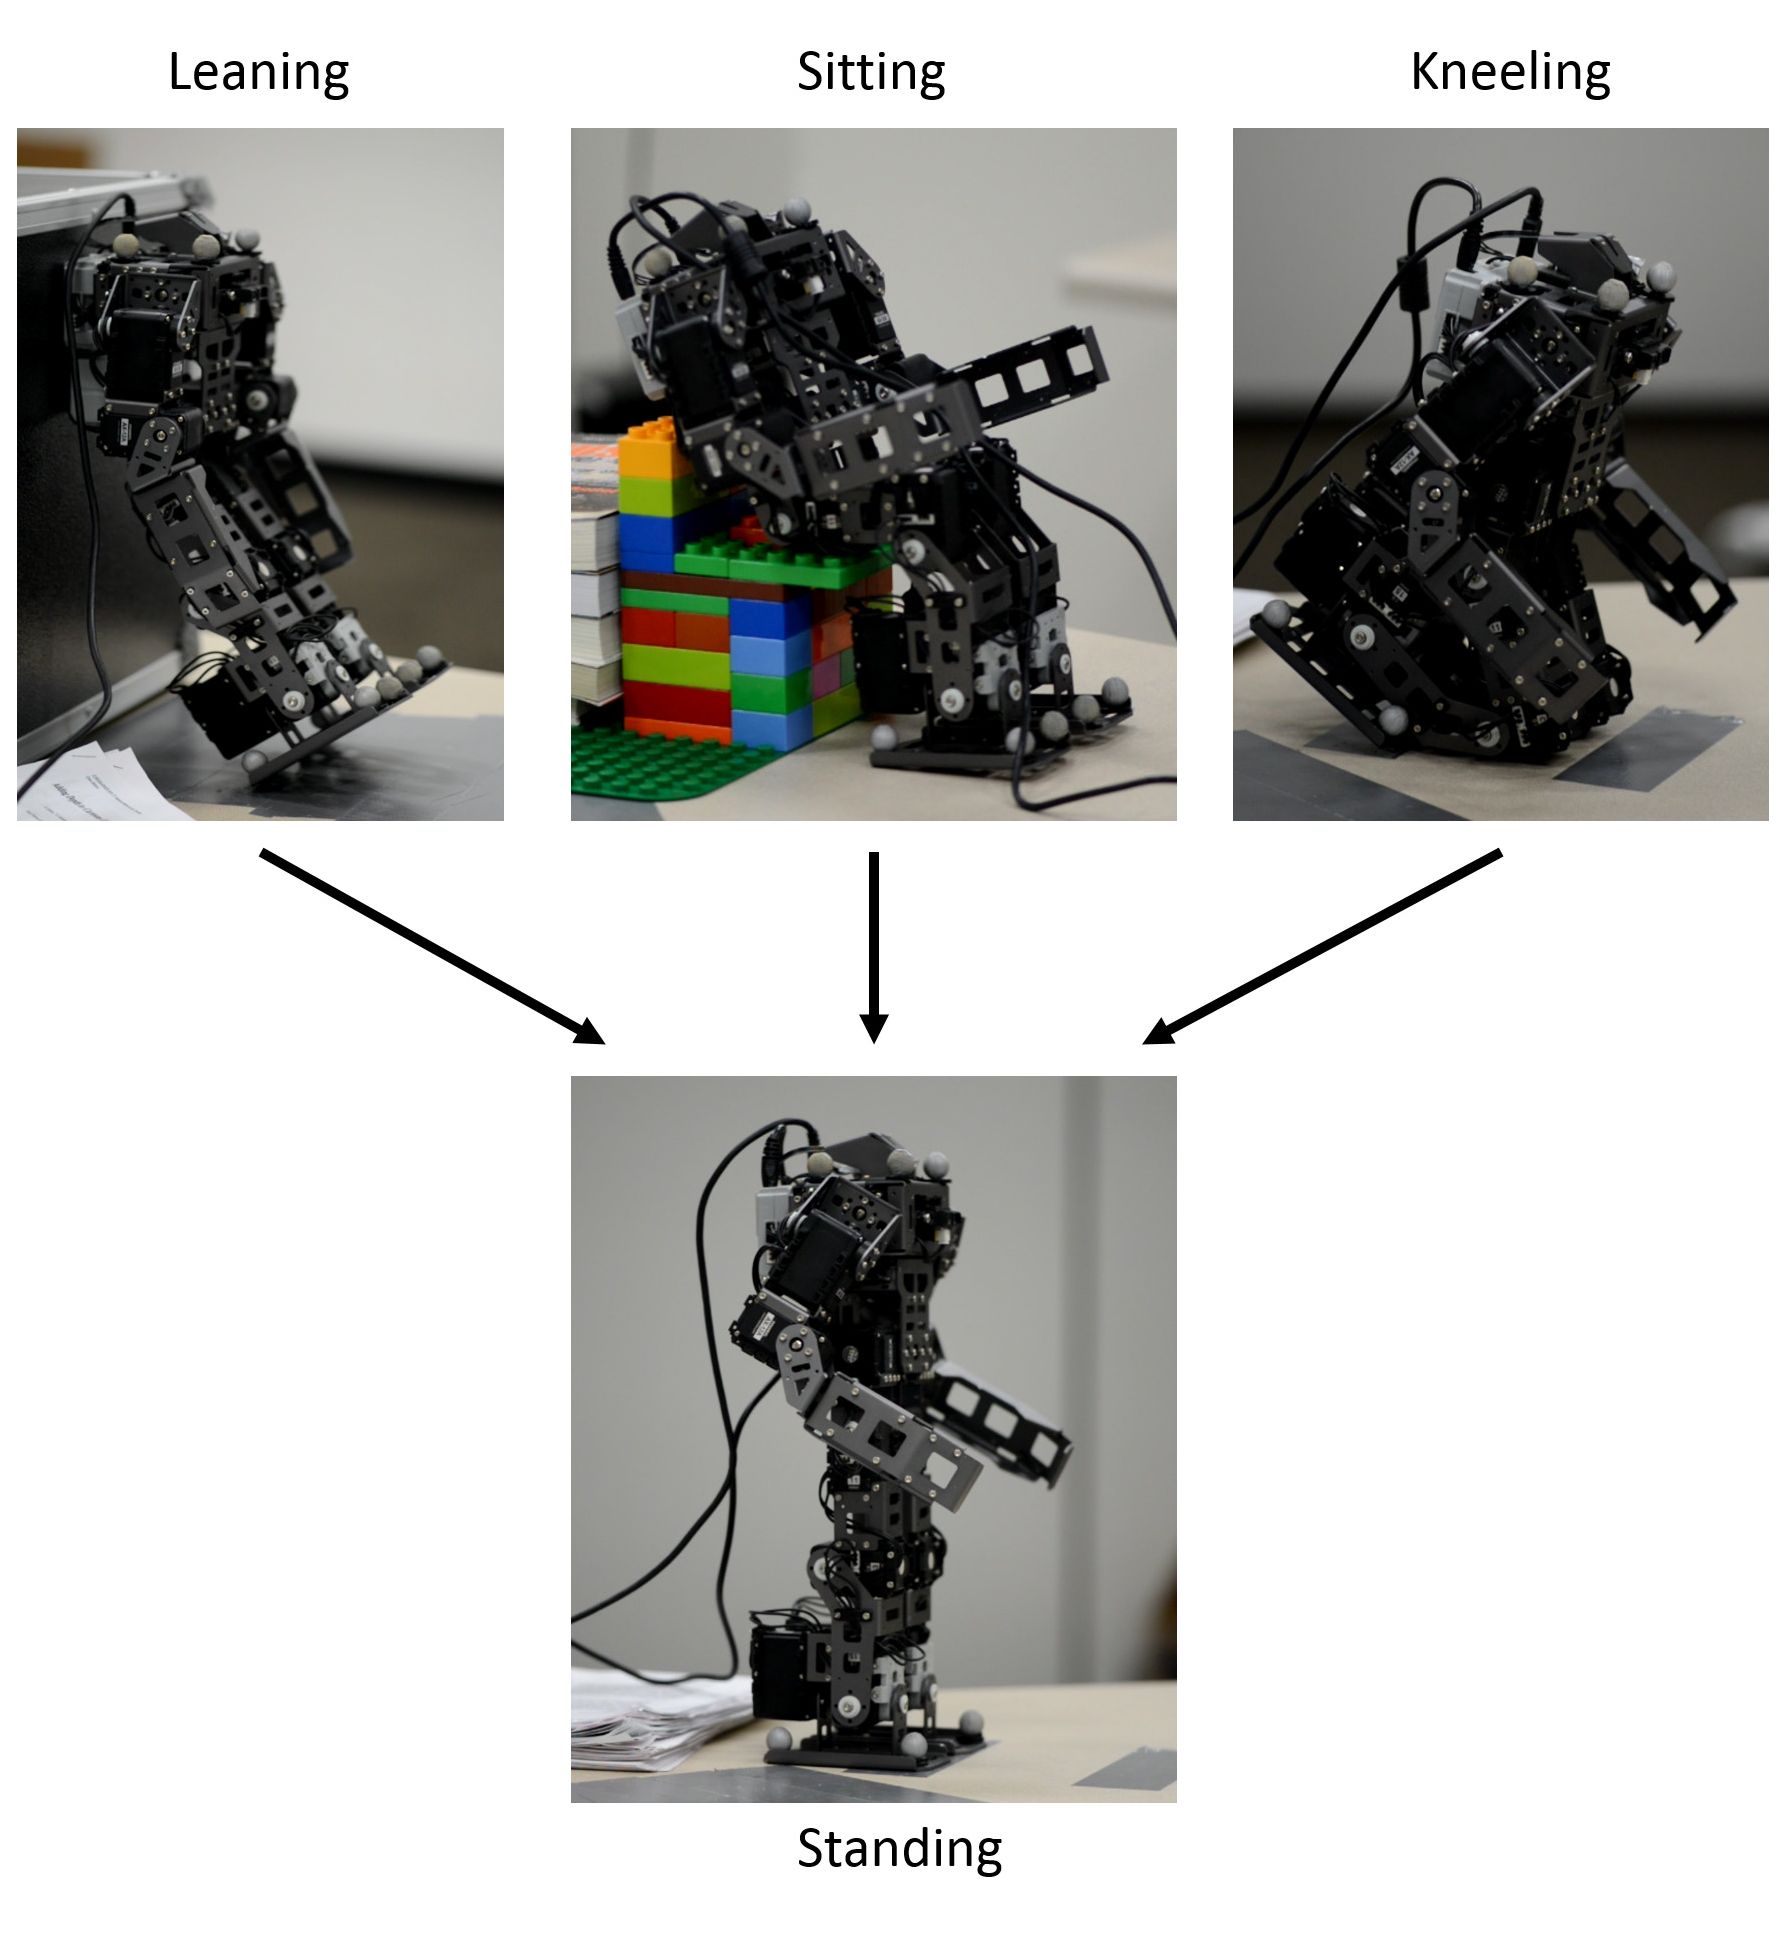
\includegraphics[width=4in]{figures/initialFinal}
  \caption{The initial and the final joint configuration of the locomotion tasks. Top row: the initial poses of leaning, sitting and kneeling. Bottom row: the final standing pose for all three tasks.}
  \label{fig:task}
\end{figure}


We first formulate a trajectory optimization problem for each task.
\begin{align}
 \label{eqn:obj}&\min_{\bar{\mathbf{q}}(t)} E_{ctrl}(\mathbf{x}(t))\\
\nonumber  \mathrm{subject\;} &\mathrm{to} \\
\label{eqn:dyn1} & \mathbf{M}(\mathbf{x})\mathbf{\ddot{x}}+\mathbf{C}(\mathbf{x},\mathbf{\dot{x}}) =\tau + \mathbf{Jf}\\
\label{eqn:dyn2} &\tau =
  \left\{
    \begin{array}{ll}
      \tau_{min} & \text{if }\tau < \tau_{min},\\
      \tau_{max} & \text{if }\tau > \tau_{max},\\
      k_p(\mathbf{q}-\bar{\mathbf{q}}) + k_d\dot{\mathbf{q}} + k_c\sgn(\dot{\mathbf{q}}) & \text{otherwise.}\\
    \end{array}
  \right.\\
\label{eqn:boundary1}&\bar{\mathbf{x}}(0) = \mathbf{x}_0\\
\label{eqn:boundary2}&\bar{\mathbf{q}}(t) = \mathbf{q}_T, \text{if } t \geq T
\end{align}

This optimization searches for a trajectory of desired joint configuration $\bar{\mathbf{q}}(t)$ that minimizes a balance related objective function (eq.(\ref{eqn:obj})), and subject to physical constraints (eq.(\ref{eqn:dyn1}) and (\ref{eqn:dyn2})) and boundary conditions (eq.(\ref{eqn:boundary1}) and (\ref{eqn:boundary2})). $\mathbf{x}_0$ is the initial condition, and $\mathbf{q}_T$ is the final pose (Figure \ref{fig:task}), both of which are provided by the user. Note that although we can specify the global translation $\mathbf{p}_0$, rotation $\mathbf{r}_0$ and joint angles $\mathbf{q}_0$ in the initial condition, we can only specify the desired joint angles for the final state because the global translation and rotation are determined by the physical simulation.

With a reasonably chosen actuator gains, the robot can alway achieve the final pose. In this case, the criterion of success for all the tasks is whether the robot remain upright at the end of its motion. We use the following objective function to encapsulate motions that can maintain an upright orientation.

\begin{equation}
  E_{ctrl}(\mathbf{q}(t))=\int_0^{T+1} -\frac{1}{\alpha(t)+\epsilon}\mathrm{d}t
  \label{eqn:controllerObj}
\end{equation}
where $\alpha(t)$ is the angle between the up direction between in the local frame of the robot's root and in the global frame $(0,0,1)$. It measures whether the robot falls out of balance. $\epsilon$ is a small positive number to prevent the denominator being zero. We choose $\epsilon=0.1$ in all our tasks. The upper limit of the integration is $T+1$, where $T$ is the duration of the entire rising motion. The extra one second is to wait the robot to settle down. We use the time horizon $T+1$ because it is still possible that the robot can fall during the settling down phase and our objective function needs to penalize this situation.

There are two main difficulties to solve the above optimization directly. First, the number of variables is large. Since our robot has 16 degrees of freedom and a rising motion can often take more than two seconds, the above space-time optimization problem can have more than 1000 variables. To solve the this problem, we use keyframes $\bar{\mathbf{q}}_1, \bar{\mathbf{q}}_2, ..., \bar{\mathbf{q}}_n$ to represent the trajectories of the desired poses $\bar{\mathbf{q}}(t)$. In between the keyframes, we linearly interpolated the poses from two adjacent keyframes. With this simplification, the \emph{control parameters} that we need to optimize consist a few keyframes and the time interval between two adjacent keyframes rather of a large number of poses for the entire trajectory. We further halve the search dimension by exploiting the symmetry of the motion. We find that all three tasks can be achieved with symmetric motions. Thus we constrain that the joint motions on the left bodies mirrors those of the right bodies. In addition, we hope that the controller can use agile lower-body motions to stand up instead of using the help from hands. For this reason, the freeze the joints at the shoulders and the elbows. This focus the controller to the motions of the lower body, which further reduces the size of the optimization problem.

The second difficulty is that during the motion, discrete contact events can happen frequently. They invalidate the gradient information, which imposes additional challenges for the continuous optimization algorithms. We choose to use Covariance Matrix Adaptation (CMA) \cite{Hansen:2009}, which can handle discontinous contacts, to optimize the control parameters. Starting from an initial Gaussian distribution, CMA samples this distribution for a set of control parameters, evaluates them using physical simulations, discards the inferior samples and updates the distribution according to the remaining good samples. With a number of iterations, the distribution moves and shrinks, and eventually converges to a good controller parameter that can successfully fulfill the task in the simulation.

\section{Simulation Calibration}

Although the optimal controllers $\bar{\mathbf{u}}(t)$ can work effectively in the simulation, they may fail to achieve the tasks when used on the robot due to the Reality Gap. To cross this gap, we develop a simulation calibration subsystem, whose goal is to improve the simulation accuracy, which would significantly increase the chance that the controller can be successfully transfered to the real robot. In this subsystem, we formulate an optimization (eq.~(\ref{eqn:calibration})) that searches for the \emph{simulation parameters} $\mathbf{\theta}$ so that the \emph{discrepancy} $E_{cali}$ is minimized between the simulated results and the robot performance in the real environment.

\begin{equation}
 \min_{\mathbf{\theta}} E_{ctrl}
\label{eqn:calibration}
\end{equation}

Many parameters $\mathbf{\theta}$ need to be set before a physical simulation starts, for example, the mass, the moment of inertia, the center of mass of each body, the coefficient of restitution, the coefficient of Coulomb friction, the gains of the actuator and many more. Changing simulation parameters can drastically alter the results of physical simulations. The accuracy of a physical simulation highly depends on the accuracy of these parameter settings. Simulation parameters are often set based on the estimation from experience, the specification of the robot, and the measurement from experiments. In our experiments, we find that many of the parameters are inaccurate. For example, the total mass of the robot is less than 1.1kg according to the CAD file while our own measurement is around 1.5kg. The height of center of mass differs more than 1cm between CAD file and our measurement. This difference in parameters could be due to the manufacturing errors and the weight of cables, glues, nuts and bolts that were used in assembling the robot. Instead of fixing the simulation parameters, we decide to adjust them during simulation calibration in order to make the simulation more accurate.

We improve the simulation accuracy by minimizing the discrepancy $E_{ctrl}$, which is defined as the difference between the state trajectories in simulations and those collected in real robot experiments. Recall that our entire algorithm is an iterative process. At the $n$th iteration, controller optimization outputs the optimal controller $\bar{\mathbf{u}}_n(t)$. We execute this controller on the robot for a number of times and compute the average state trajectory $\tilde{\mathbf{x}}_n(t)$ of the robot motion. We use the average of the multiple trajectories because we find that even with the same controller, we can get slightly different trajectories due to the varied initial condition, the noise from the sensor, from the actuator and from the environment. Together with the $n-1$ pairs of controllers and their associated average state trajectories from previous iterations, we can compute the discrepancy using the following expression. 

\begin{equation}
  E_{cali}=\frac{1}{n}\sum_{i=1}^{n}\int_{0}^{T+1}||\tilde{\mathbf{x}}_i(t)-\mathbf{x}_i(t)||_{\mathbf{W}}^2\mathrm{d}t
  \label{eqn:calibrationObj}
\end{equation}
where $\mathbf{x}(t)$ and $\tilde{\mathbf{x}}(t)$ are state trajectories in the simulation and in the real world respectively. $\mathbf{W}$ is a diagonal matrix, which weights the relative importance of each joint. Due to the complex interplay between the simulation results and the simulation parameters, the optimization (\ref{eqn:calibration}) is nonlinear and nonconvex.  Our numerical experiments show that the objective function has many local minima, which can impose difficulties to gradient based optimization algorithms. Similar to controller optimization, we choose to use CMA for the optimization. In this case, each CMA sample is a candidate set of simulation parameters $\mathbf{\theta}$. To evaluate each CMA sample, we set the parameters into the physical simulator, simulate the robot motion $\mathbf{x}(t)$, and then compute the objective function eq. (\ref{eqn:calibrationObj}).

In our work, we initialize the simulation parameters as follows. We set the physical properties of each body, including the mass, the moment of inertia and the COM according to the CAD files. We set the actuator gains based on the measurement from experiments. We leave all other parameters as default values in DART. Although these parameters are not accurate, they serve as a pretty good initial guess. During simulation calibration, we search the parameter space within a bounded range centered at the initial guess. In addition, we also employ two simplifications to speed up the optimization. First, we narrow down the simulation parameters to include only the actuator gains of each servo and the COM of each body. Since each task is to achieve a specific final pose while keeping balance, we believe that the actuator gains and the COM's are the two most important simulation parameters. Accurate actuator gains determines whether the robot can reach and hold the final pose, and correct COM's play an important role in balance control. This manual feature selection drastically reduce the search space of the optimization. Second, we zero out most of the diagonal entries of $\mathbf{W}$ in eq. (\ref{eqn:calibrationObj}) except for the rows corresponding to the global orientation. More specifically, we simply measure the discrepancy based solely on $\alpha$, the angle between the up direction between in the local frame of the robot's torso and in the global frame $(0,0,1)$.

\begin{equation}
  E_{cali}=\frac{1}{n}\sum_{i=1}^{n}\int_{0}^{T+1}(\tilde{\alpha}_i(t)-\alpha_i(t))^2\mathrm{d}t
  \label{eqn:calibrationObj1}
\end{equation}

The objective function eq. (\ref{eqn:calibrationObj1}) captures the most important features that characterize the success or failure of our tasks (see eq.(\ref{eqn:controllerObj})), and eliminates the potentially tedious manual tuning of the weight matrix $\mathbf{W}$.





\section{Results}

\begin{figure}[!t]
  \centering
  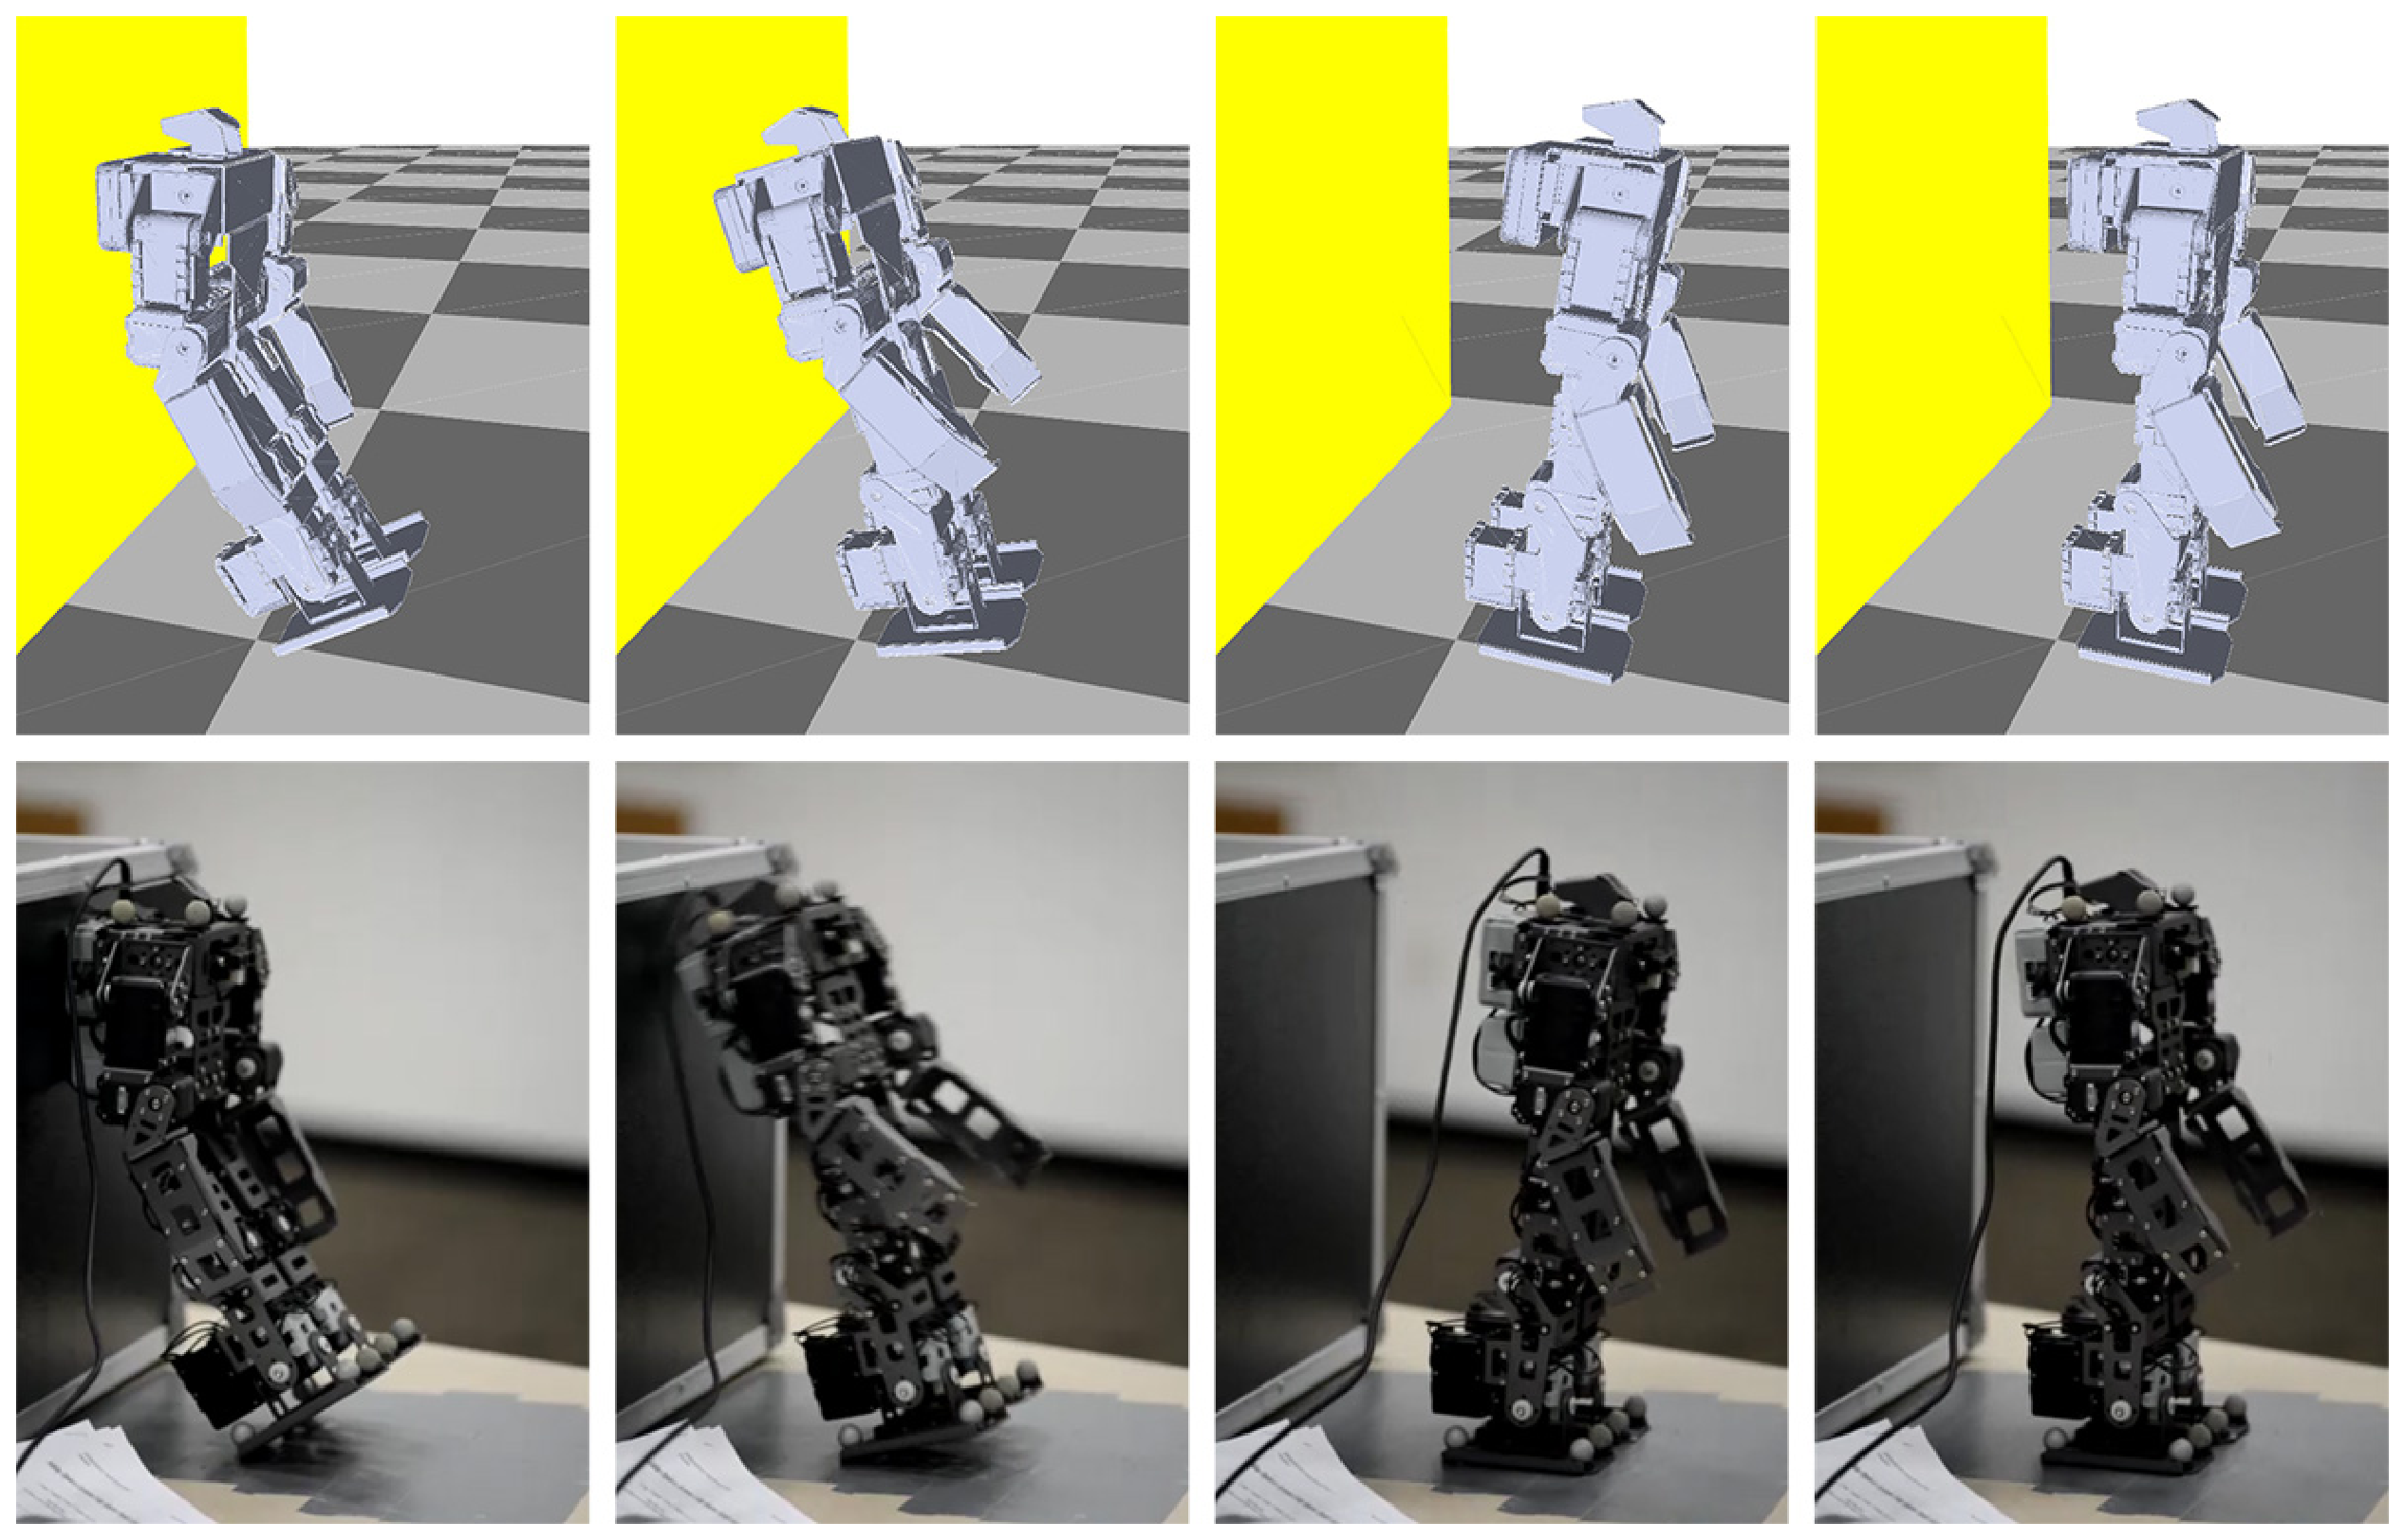
\includegraphics[width=0.7\textwidth]{figures/lean2Stand}
  \caption{The results of the lean-to-stand task in the simulation and on the real robot.}
  \label{fig:lean2Stand}
\end{figure}

\begin{figure}[!t]
  \centering
  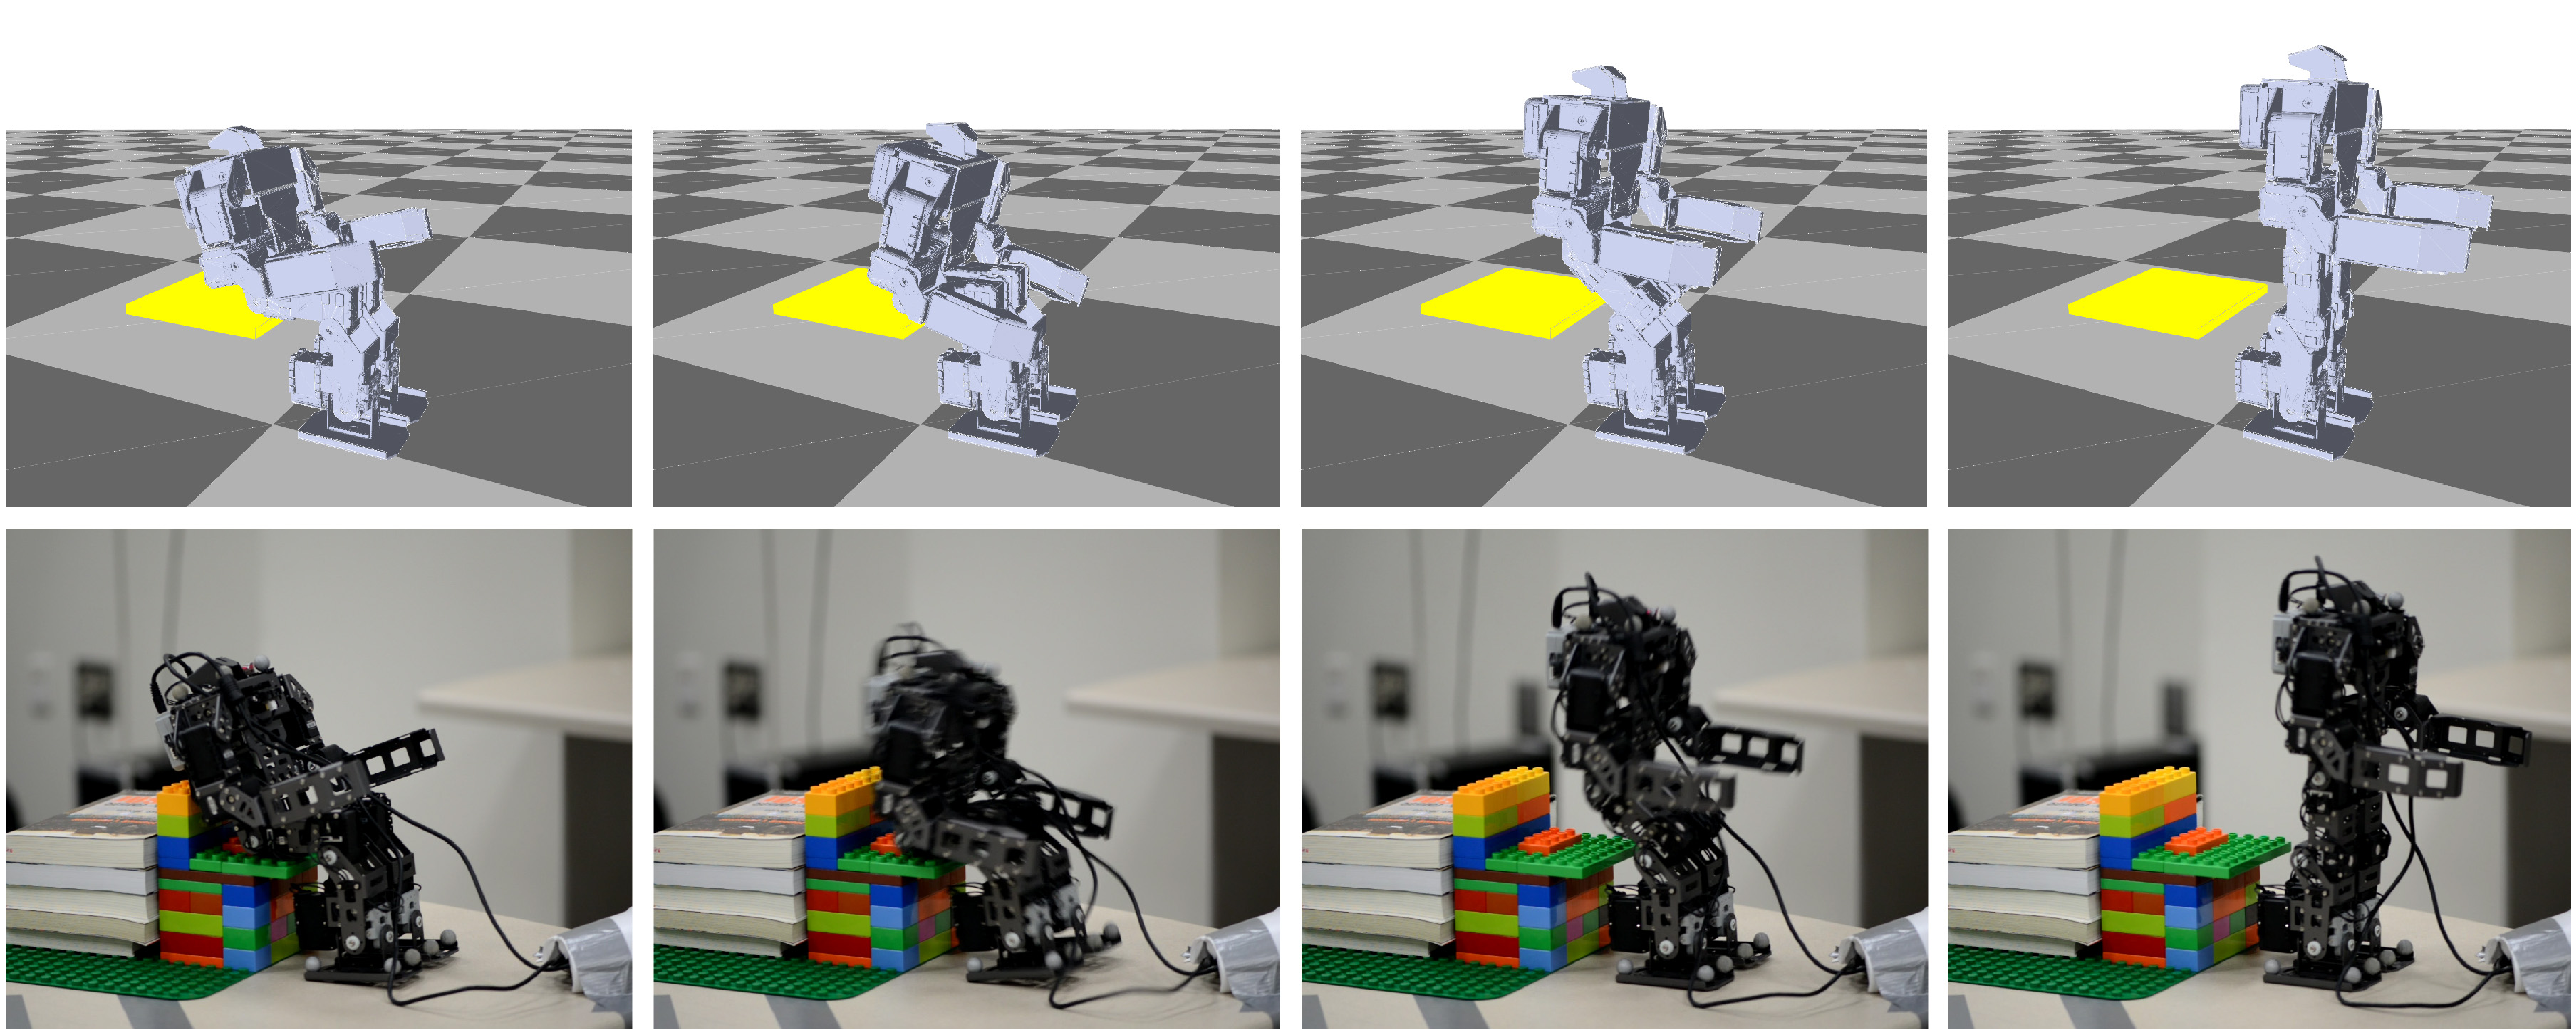
\includegraphics[width=\textwidth]{figures/sit2Stand}
  \caption{The results of the sit-to-stand task in the simulation and on the real robot.}
  \label{fig:lean2Stand}
\end{figure}

\begin{figure}[!t]
  \centering
  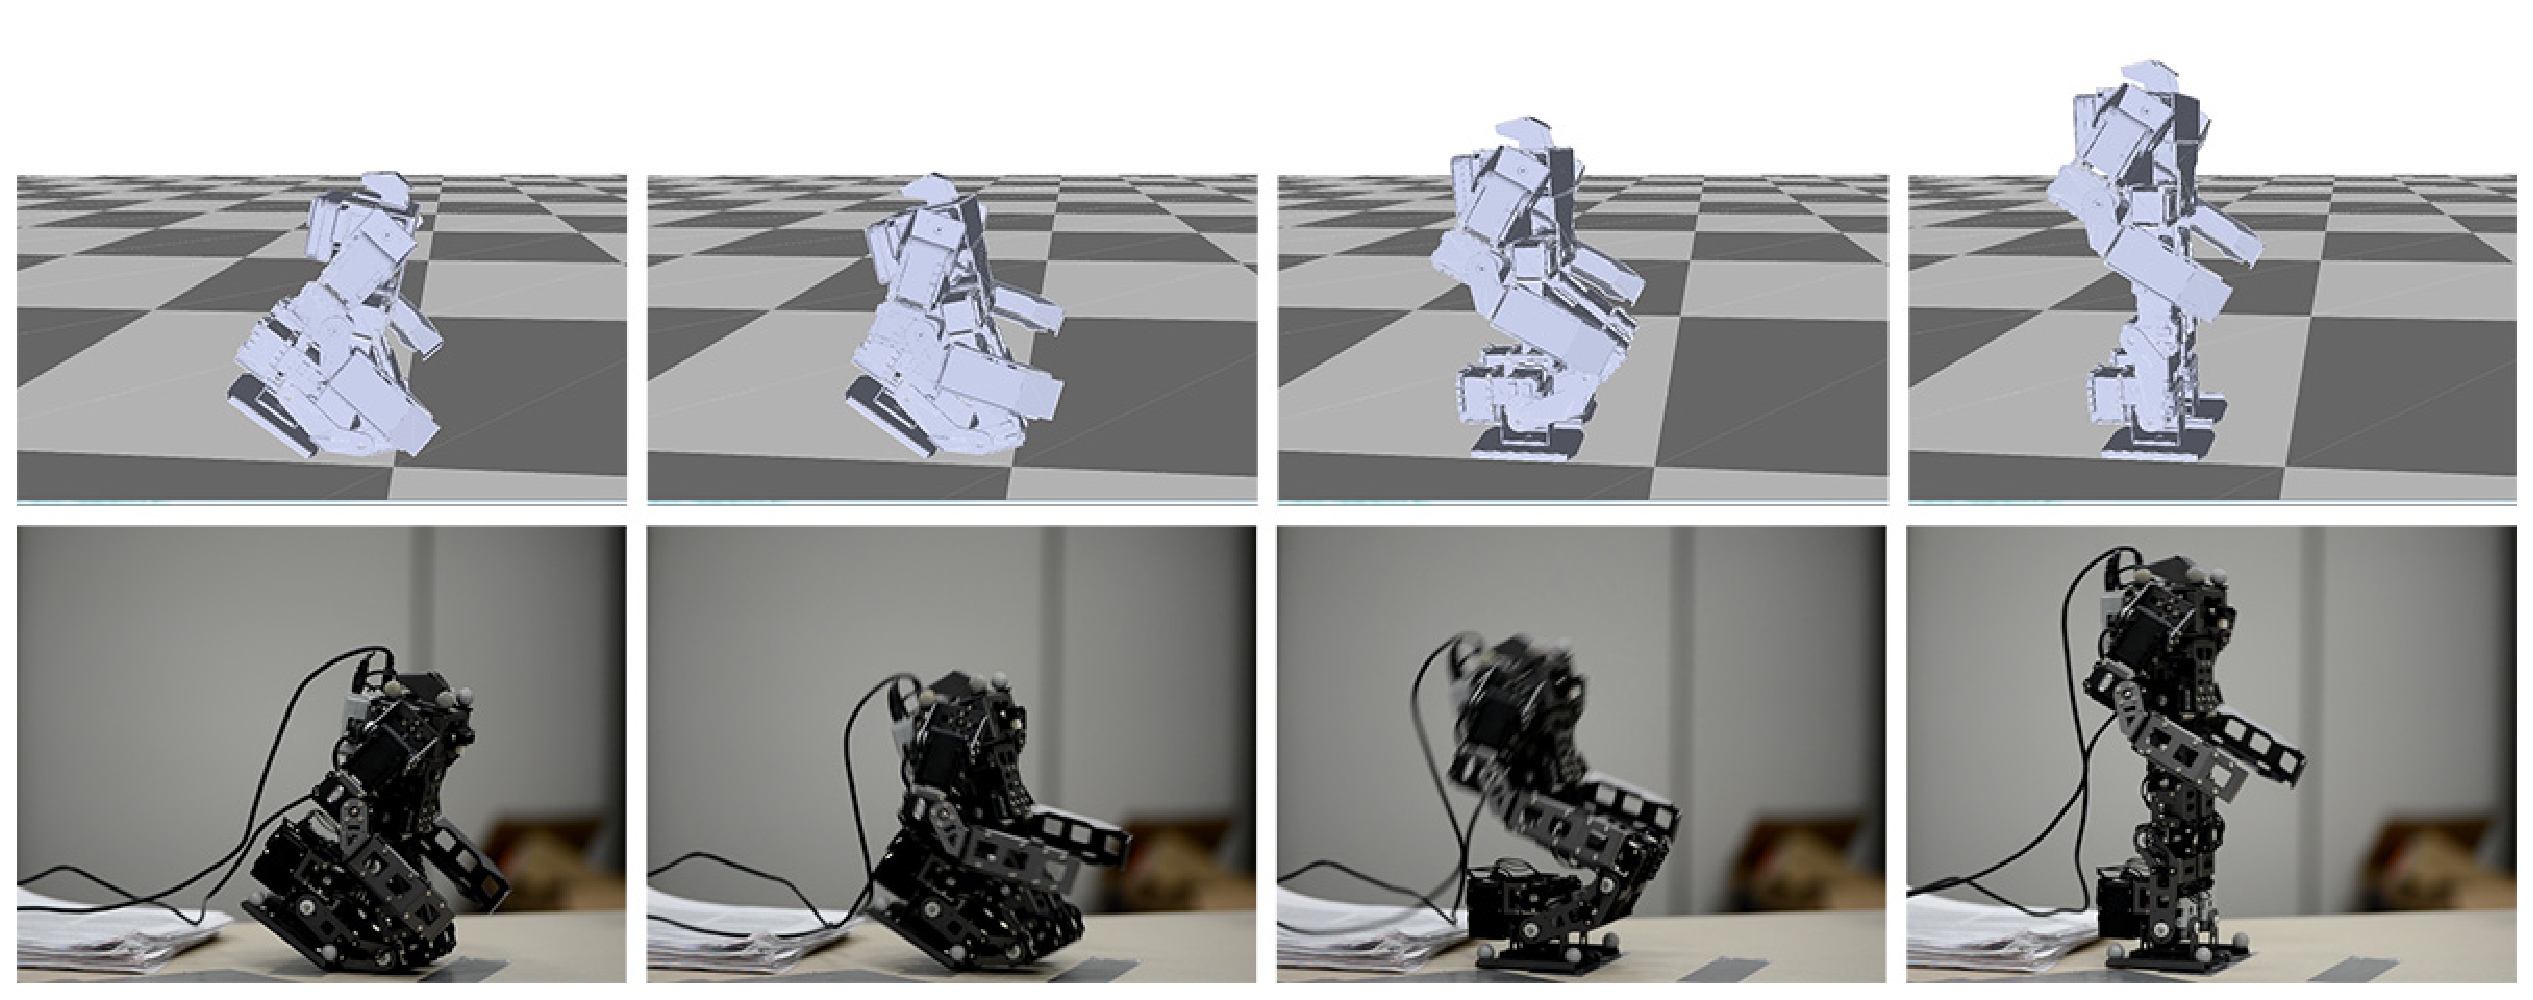
\includegraphics[width=\textwidth]{figures/kneel2Stand}
  \caption{The results of the kneel-to-stand task in the simulation and on the real robot.}
  \label{fig:kneel2Stand}
\end{figure}

\section{Discussion}
